\documentclass{article}
\usepackage{graphicx} % Required for inserting images
\usepackage{tikz}
\begin{document}

\begin{center}

\large Grafo de Errera. \vspace{2cm}

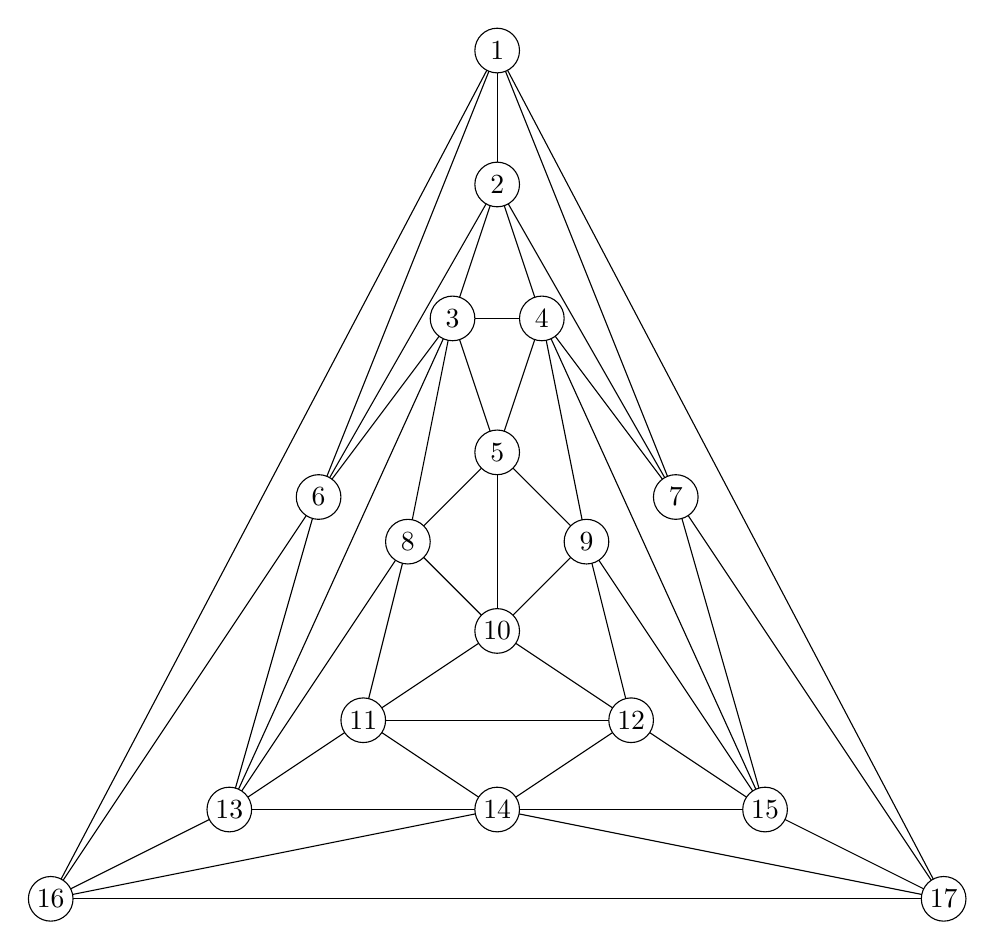
\begin{tikzpicture}[scale=0.567] % Gráfico escalado a 67% para ajustarse a la página
  \draw (0,10) -- (0,7);
  \draw (0,7) -- (-1,4);
  \draw (-1,4) -- (0,1);
  \draw (0,-3) -- (-3,-5);
  \draw (-3,-5) -- (-6,-7);
  \draw (0,7) -- (1,4);
  \draw (1,4) -- (0,1);
  \draw (0,-3) -- (3,-5);
  \draw (3,-5) -- (6,-7);
  \draw (-3,-5) -- (3,-5);
  \draw (0,-3) -- (0,1);
  \draw (1,4) -- (-1,4);
  \draw (-4,0) -- (0,10);
  \draw (0,10) -- (4,0);
  \draw (0,7) -- (-4,0);
  \draw (0,7) -- (4,0);
  \draw (-1,4) -- (-4,0);
  \draw (1,4) -- (4,0);
  \draw (-2,-1) -- (0,1);
  \draw (0,1) -- (2,-1);
  \draw (2,-1) -- (0,-3);
  \draw (0,-3) -- (-2,-1);
  \draw (-2,-1) -- (-1,4);
  \draw (1,4) -- (2,-1);
  \draw (-6,-7) -- (-4,0);
  \draw (4,0) -- (6,-7);
  \draw (6,-7) -- (2,-1);
  \draw (-2,-1) -- (-6,-7);
  \draw (-3,-5) -- (-2,-1);
  \draw (2,-1) -- (3,-5);
  \draw (-3,-5) -- (0,-7);
  \draw (0,-7) -- (3,-5);
  \draw (0,-7) -- (-6,-7);
  \draw (0,-7) -- (6,-7);
  \draw (-10,-9) -- (0,10);
  \draw (0,10) -- (10,-9);
  \draw (10,-9) -- (6,-7);
  \draw (-6,-7) -- (-10,-9);
  \draw (-10,-9) -- (0,-7);
  \draw (0,-7) -- (10,-9);
  \draw (10,-9) -- (-10,-9);
  \draw (-10,-9) -- (-4,0);
  \draw (4,0) -- (10,-9);
  \draw (1,4) -- (6,-7);
  \draw (-6,-7) -- (-1,4);
  \draw[fill=white](0,10)circle(0.5)node[]{1};
  \draw[fill=white](0,7)circle(0.5)node[]{2};
  \draw[fill=white](-1,4)circle(0.5)node[]{3};
  \draw[fill=white](1,4)circle(0.5)node[]{4};
  \draw[fill=white](0,1)circle(0.5)node[]{5};
  \draw[fill=white](-4,0)circle(0.5)node[]{6};
  \draw[fill=white](4,0)circle(0.5)node[]{7};
  \draw[fill=white](-2,-1)circle(0.5)node[]{8};
  \draw[fill=white](2,-1)circle(0.5)node[]{9};
  \draw[fill=white](0,-3)circle(0.5)node[]{10};
  \draw[fill=white](-3,-5)circle(0.5)node[]{11};
  \draw[fill=white](3,-5)circle(0.5)node[]{12};
  \draw[fill=white](-6,-7)circle(0.5)node[]{13};
  \draw[fill=white](0,-7)circle(0.5)node[]{14};
  \draw[fill=white](6,-7)circle(0.5)node[]{15};
  \draw[fill=white](-10,-9)circle(0.5)node[]{16};
  \draw[fill=white](10,-9)circle(0.5)node[]{17};
\end{tikzpicture}

\end{center}
\end{document}
